\documentclass{beamer}

\usepackage{hyperref}

\usepackage{tcolorbox}
\tcbuselibrary{theorems}

\newtcolorbox{MyBox}[2][]{
  colback=red!5,
  colframe=red!75!black,
  title=#2,
  #1
}

\usepackage{focs-slides}

\usepackage{color} %red, green, blue, yellow, cyan, magenta, black, white
\definecolor{mygreen}{RGB}{28,172,0} % color values Red, Green, Blue
\definecolor{mylilas}{RGB}{170,55,241}

\title{Wavelet Encoding}
\author{Yinan Dong, Jingkai Zhang, Letian Zheng}
\date{Spring 2024}
\course{image/MATH214}

\definecolor{darkblue}{HTML}{6666dd} 
\definecolor{darkslategray}{HTML}{2f4f4f} 
%\colortheme{green!42!black}
%\colortheme{orange!85!black}
%\colortheme{darkblue}
%\colortheme{pink!80!black}
%\colortheme{orange!85!white!90!black}
%\colortheme{darkslategray}

\usepackage{listings}
\lstset{language=Matlab,
    %basicstyle=\color{red},
	basicstyle=\ttfamily\scriptsize
    breaklines=true,%
    morekeywords={matlab2tikz},
    keywordstyle=\color{blue},
    morekeywords=[2]{1}, keywordstyle=[2]{\color{black}},
    identifierstyle=\color{black},
    stringstyle=\color{mylilas},
    commentstyle=\color{mygreen},
    showstringspaces=false,%without this there will be a symbol in the places where there is a space
	showtabs=false
    numbers=left,
    numberstyle={\tiny \color{black}},% size of the numbers
    numbersep=9pt, % this defines how far the numbers are from the text
    emph=[1]{for,end,break},emphstyle=[1]\color{red}, %some words to emphasise
    %emph=[2]{word1,word2}, emphstyle=[2]{style},    
}

\begin{document}

\maketitle

% table of contents
%\toc{enum}
%\toc{mindmap}
\section{Introduction}

\section{Wavelet transform in compression}
\begin{frame}{Use Harr wavelet to compress a matrix}

\begin{columns}[T,onlytextwidth]

	\column{.5\textwidth}
	
	\centering
	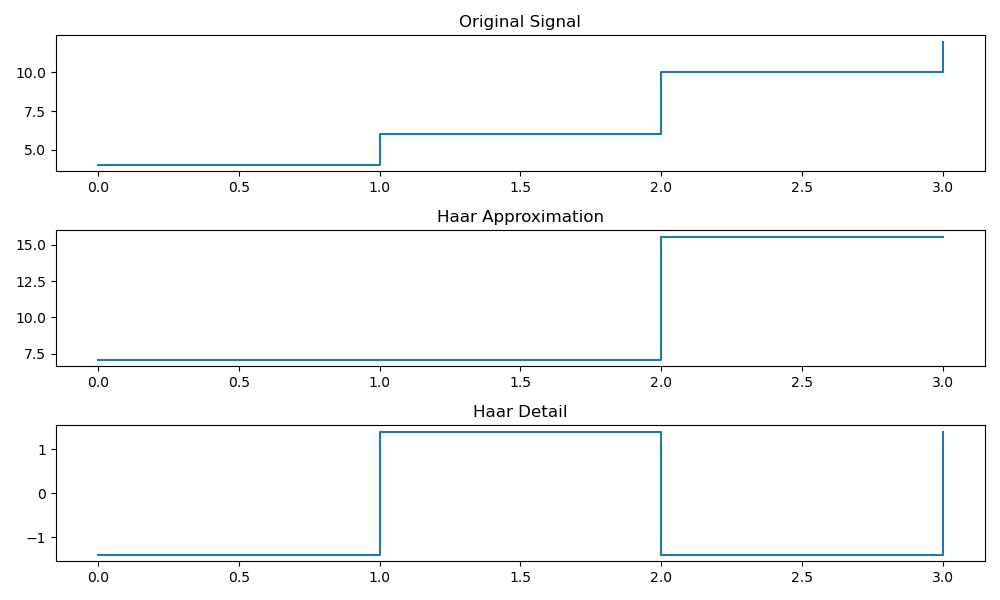
\includegraphics[width=.9\columnwidth]{image/haar_1}
	\column{.5\textwidth}
	\begin{theorem}
		\text{Define} \begin{equation} \psi (n)=\left \{
		\begin{aligned}
		 \frac{1}{2} \quad 1 \leq n \leq 2\\
		-\frac{1}{2} \quad 3 \leq n \leq 4\\
		0 \quad otherwise\\
		\end{aligned} 
		\right 
		.
		\end{equation}\\
		\text{and} $\quad \psi_{j,k} (x)=\psi(2^jx-k).$
\end{theorem}
\end{columns}

\end{frame}



\begin{frame}{Use Harr wavelet to compress a matrix}
For a matrix $A \in\ M_8$,
\small
{
\[
H_1 = \left(\begin{array}{cccccccc}
\frac{1}{2} & 0 & 0 & 0 & \frac{1}{2} & 0& 0& 0\\
\frac{1}{2} & 0 & 0 & 0 & -\frac{1}{2} & 0& 0& 0 \\
0 & \frac{1}{2} & 0 & 0 & 0 & \frac{1}{2}& 0& 0 \\
0 & \frac{1}{2} & 0 & 0 & 0 & -\frac{1}{2}& 0& 0 \\
0&0 & \frac{1}{2} & 0 & 0 & 0 & \frac{1}{2}& 0 \\
0&0 & \frac{1}{2} & 0 & 0 & 0 & -\frac{1}{2}& 0 \\
0&0&0 & \frac{1}{2} & 0 & 0 & 0 & \frac{1}{2}\\
0&0&0 & \frac{1}{2} & 0 & 0 & 0 & -\frac{1}{2}
\end{array}\right)
\]
\[
H_2=\left(\begin{array}{cccccccc}
\frac{1}{2} & 0 & \frac{1}{2} & 0 & 0 & 0& 0& 0\\
\frac{1}{2} & 0 & -\frac{1}{2} & 0 & 0 & 0& 0& 0 \\
0 & \frac{1}{2} & 0 & \frac{1}{2} & 0 & 0& 0& 0 \\
0 & \frac{1}{2} & 0 & -\frac{1}{2} & 0 & 0& 0& 0 \\
0&0 & 0 & 0 & 1 & 0 & 0& 0 \\
0&0 & 0 & 0 & 0 & 1 & 0& 0 \\
0&0&0 & 0 & 0 & 0 & 1 & 0\\
0&0&0 & 0 & 0 & 0 & 0 & 1
\end{array}\right)
\]
}
\end{frame}

\begin{frame}{Use Harr wavelet to compress a matrix}
\[
H_3 = \left(\begin{array}{cccccccc}
\frac{1}{2} & \frac{1}{2} & 0 & 0 & 0 & 0& 0& 0\\
\frac{1}{2} & -\frac{1}{2} & 0 & 0 & 0 & 0& 0& 0 \\
0 & 0 & 1 & 0 & 0 & 0 & 0 & 0 \\
0 & 0 & 0 & 1 & 0 & 0 & 0 & 0 \\
0 & 0 & 0 & 0 & 1 & 0 & 0 & 0 \\
0 & 0 & 0 & 0 & 0 & 1 & 0 & 0 \\
0 & 0 & 0 & 0 & 0 & 0 & 1 & 0 \\
0 & 0 & 0 & 0 & 0 & 0 & 0 & 1
\end{array}\right)
\quad \quad 
\]

\medskip \medskip

\[
H = H_1H_2H_3, B = H^TAH
\]

\end{frame}

\begin{frame}{Use Harr wavelet to compress a matrix}
$\text{Choose a $\epsilon$ and turn every element in the matrix smaller than it into 0.}$

$\text{Denote this new matrix as $B',\ A'=(H^T)^{-1}B'(H)^{-1}$}$

$\text{In this way, we successfully compress matrix A.}$

\medskip

$\text{If $H_1,H_2,H_3$ is turned into orthogonal matrixes, }$
$\text{the compression will be of better quality.}$
\end{frame}

\section{Experiment}

\begin{frame}{Method}

\begin{MyBox}{Experiment Target}
	Utilize wavelet encoding method the compress image.
\end{MyBox}
		
\medskip

\textbf{Simplification}: In the experiment, we first convert the sample images into grayscale before compressing them. This approach reduces the amount of data and simplifies the processing, thereby enhancing the efficiency of compression. \\

\medskip

\textbf{Metrics for measuring the degree of image compression}: 
\begin{enumerate}
	\item Comparison of image size before and after compression
	\item Comparison of image file size before and after compression
	\item Peak signal-to-noise ratio (PSNR)
\end{enumerate}

\end{frame}

\begin{frame}{Procedure}
	\begin{enumerate}
		\item \textbf{Initialization}: The original image is loaded into the program from a file. If the image is in color, it may be converted to grayscale to simplify the compression process.
		\item \textbf{Preprocessing}: The image is processed row by row and column by column, applying the Haar wavelet transform. This step decomposes the image into a set of wavelet coefficients that represent the image in the wavelet domain.
		\item \textbf{Quantization and Thresholding}: Wavelet coefficients are modified to compress the image data. Coefficients below a certain threshold are set to zero, effectively reducing the amount of data.
		\item \textbf{Inverse Wavelet Transform}: An inverse wavelet transform is applied to the modified coefficients to reconstruct a compressed version of the original image.
		\item \textbf{Performance Analysi}: After compression, metrics can be calculated to evaluate the quality and efficiency of the compression.
	\end{enumerate}
\end{frame}





\begin{frame}[fragile]{Codes for Wavelet Transformation}
	\lstinputlisting{../src/haar_wavelet_transform.m}
\end{frame}

\begin{frame}[fragile]{Codes for Inversed Wavelet Transformation}
	\lstinputlisting{../src/ihaar_wavelet_transform.m}
\end{frame}

\begin{frame}{Results}

\begin{columns}[T,onlytextwidth]

	\column{.5\textwidth}
	
	\centering
	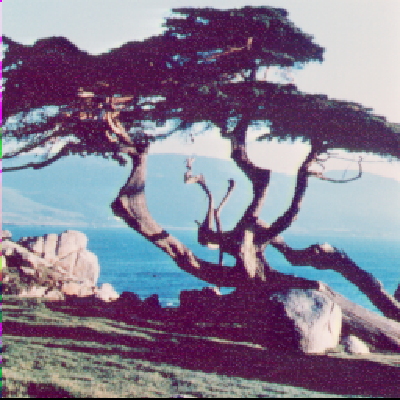
\includegraphics[page=1, width=.7\columnwidth]{image/images}

	\includegraphics[page=2, width=.7\columnwidth]{image/images}

	\column{.5\textwidth}

	\begin{MyBox}{Original image}
		\footnotesize{
		Image Size: 65536 bytes \\
		Image File Size: 43632 bytes
		}
	\end{MyBox}

	\medskip \medskip \medskip \medskip \medskip \medskip \medskip 

	\begin{MyBox}{Threshold: 20}
		\footnotesize{
		PSNR value: 33.4615 dB \\
		Image Memory Size: 65536 bytes \\
		Image File Size: 25706 bytes
		}
	\end{MyBox}

\end{columns}
		
\end{frame}

\begin{frame}{Results}

	\begin{columns}[T,onlytextwidth]
	
		\column{.5\textwidth}
		
		\centering
		\includegraphics[page=3, width=.7\columnwidth]{image/images}
	
		\includegraphics[page=5, width=.7\columnwidth]{image/images}
	
		\column{.5\textwidth}
	
		\begin{MyBox}{Threshold: 40}
			\footnotesize{
			PSNR value: 29.6200 dB \\
			Image Memory Size: 65536 bytes \\
			Image File Size: 20288 bytes
			}
		\end{MyBox}
		
		\medskip \medskip \medskip \medskip \medskip \medskip 

		\begin{MyBox}{Threshold: 100}
			\footnotesize{
			PSNR value: 22.1378 dB \\
			Image Memory Size: 65536 bytes \\
			Image File Size: 15667 bytes
			}
		\end{MyBox}


	\end{columns}
			
	\end{frame}

\begin{frame}{Reference}
	Reference: 
	\begin{enumerate}
		\item \href{https://en.wikipedia.org/wiki/Wavelet_transform}{Wavelat Transformation, Wikipedia} 
		\item \href{https://en.wikipedia.org/wiki/Haar_wavelet}{Haar Wavelat, Wikipedia} 
	\end{enumerate}

	\medskip \medskip

	Complete code can be found in the following \href{https://github.com/zlt-0503/Wavelet-Compression}{Github repository} 
\end{frame}

\thankframe

\end{document}
